\newif\ifsolutions
\solutionstrue % Show solutions
%\solutionsfalse % Hide solutions

\documentclass{article}
\usepackage{geometry}
\geometry{margin=1in}
\usepackage{tikz}
\usepackage{amssymb}

% fleqn allows setting indent of display math
\usepackage[fleqn]{amsmath}
\setlength{\mathindent}{0pt} % Set indent
% Disable equation numbering (https://tex.stackexchange.com/a/360378)
\makeatletter
\renewcommand\tagform@[1]{}
\makeatother

% Allow Unicode (some, e.g., © and £ at least)
% https://tex.stackexchange.com/questions/370278/is-there-any-reason-to-use-inputenc
\usepackage[utf8]{inputenc}

% Hyperlinks
\usepackage{hyperref}
\hypersetup{colorlinks=true, urlcolor=blue, linkcolor=blue}

% Prevent indentation of paragraphs
\setlength\parindent{0pt}
\setlength{\parskip}{\baselineskip}

% Spacing above/below equations
% https://tex.stackexchange.com/a/69678
\AtBeginDocument{%
 \abovedisplayskip=-\parskip
 \abovedisplayshortskip=-\parskip
 \belowdisplayskip=0pt
 \belowdisplayshortskip=0pt
}

% Allow 3 additional subsection levels
% https://tex.stackexchange.com/a/60212
\usepackage{titlesec}
\setcounter{secnumdepth}{6}
% H4 in HTML
\titleformat{\paragraph}{\normalfont\normalsize\bfseries}{\theparagraph}{1em}{}
\titlespacing*{\paragraph}{0pt}{3.25ex plus 1ex minus .2ex}{1.5ex plus .2ex}
% H5 in HTML
\titleformat{\subparagraph}{\normalfont\normalsize\bfseries}{\thesubparagraph}{1em}{}
\titlespacing*{\subparagraph}{0pt}{3.25ex plus 1ex minus .2ex}{1.5ex plus .2ex}
% H6 in HTML
\titleformat{\subsubparagraph}{\normalfont\normalsize\bfseries}{\thesubsubparagraph}{1em}{}
\titlespacing*{\subsubparagraph}{0pt}{3.25ex plus 1ex minus .2ex}{1.5ex plus .2ex}

% So enumerate at all levels is numbers
% https://tex.stackexchange.com/questions/78842/nested-enumeration-numbering
\renewcommand{\labelenumii}{\arabic{enumii}.}
\renewcommand{\labelenumiii}{\arabic{enumiii}.}
\renewcommand{\labelenumiv}{\arabic{enumiv}.}

\renewcommand{\mbox}{\text}
\newcommand{\ds}[0]{\displaystyle}
\newcommand{\ihat}[0]{\hat{\boldsymbol{\imath}}}
\newcommand{\jhat}[0]{\hat{\boldsymbol{\jmath}}}
\newcommand{\khat}[0]{\hat{\boldsymbol{k}}}
\newcommand{\xhat}[0]{\hat{\mathbf{x}}}
\newcommand{\yhat}[0]{\hat{\mathbf{y}}}
\newcommand{\zhat}[0]{\hat{\mathbf{z}}}
\newcommand{\rhat}[0]{\hat{\mathbf{r}}}
\newcommand{\bfvec}[1]{\vec{\mathbf{#1}}}
\newcommand{\bfcdot}[0]{\boldsymbol{\cdot}}

\usepackage{fancyhdr}
\pagestyle{fancy}
\lhead{Superposition and Symmetry}
\rhead{\thepage}
\fancyfoot{}

\begin{document}

% Figures:
% https://www.mathcha.io/editor/M55KMuQLiLmH9Vgp0Ptw6QGB3HnpzJnnuM6VoB7

\section{Overview}

In previous activities, only one charge was responsible for creating the electric field. When there are more charges, superposition can be used to find the total electric field by summing $\bfvec{E}$ due to each charge. Superposition can also be used to find the total electric force on a charge due to two or more charges.

Superposition problems are often simplified by recognizing a symmetry. For example, if we want to know the electric field at the origin due to charges $+q$ at $(x,y)=(\pm a, 0)$, we can state the answer is zero without computing the fields due to each charge -- we know they will be equal and opposite.

\section{Problem}

Charge $q_1 = +q$ is at $(x, y) = (a, 0)$, charge $q_2 = +q$ is at $(x, y) = (-a, 0)$, and charge $q_3 = -q$ is at $(x, y) = (0, a)$. Assume that $q$ is a positive number.

\begin{enumerate}

  \item Draw this charge configuration below.

\end{enumerate}

\ifsolutions


\tikzset{every picture/.style={line width=0.75pt}} %set default line width to 0.75pt        

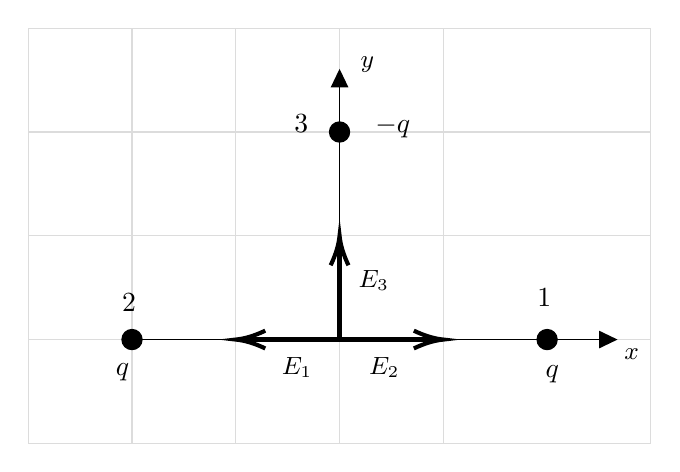
\begin{tikzpicture}[x=0.75pt,y=0.75pt,yscale=-1,xscale=1]
%uncomment if require: \path (0,200); %set diagram left start at 0, and has height of 200

%Shape: Grid [id:dp331631089200787] 
\draw  [draw opacity=0] (0,0) -- (300,0) -- (300,200) -- (0,200) -- cycle ; \draw  [color={rgb, 255:red, 220; green, 220; blue, 220 }  ,draw opacity=1 ] (50,0) -- (50,200)(100,0) -- (100,200)(150,0) -- (150,200)(200,0) -- (200,200) ; \draw  [color={rgb, 255:red, 220; green, 220; blue, 220 }  ,draw opacity=1 ] (0,50) -- (300,50)(0,100) -- (300,100)(0,150) -- (300,150) ; \draw  [color={rgb, 255:red, 220; green, 220; blue, 220 }  ,draw opacity=1 ] (0,0) -- (300,0) -- (300,200) -- (0,200) -- cycle ;
%Straight Lines [id:da14224998842180447] 
\draw    (50,150) -- (280.93,150) ;
\draw [shift={(283.93,150)}, rotate = 180] [fill={rgb, 255:red, 0; green, 0; blue, 0 }  ][line width=0.08]  [draw opacity=0] (8.93,-4.29) -- (0,0) -- (8.93,4.29) -- cycle    ;
%Straight Lines [id:da6009743108133081] 
\draw    (150,150) -- (150,22.58) ;
\draw [shift={(150,19.58)}, rotate = 90] [fill={rgb, 255:red, 0; green, 0; blue, 0 }  ][line width=0.08]  [draw opacity=0] (8.93,-4.29) -- (0,0) -- (8.93,4.29) -- cycle    ;
%Shape: Circle [id:dp897042553915123] 
\draw  [fill={rgb, 255:red, 0; green, 0; blue, 0 }  ,fill opacity=1 ] (145.13,50) .. controls (145.13,47.31) and (147.31,45.13) .. (150,45.13) .. controls (152.69,45.13) and (154.87,47.31) .. (154.87,50) .. controls (154.87,52.69) and (152.69,54.87) .. (150,54.87) .. controls (147.31,54.87) and (145.13,52.69) .. (145.13,50) -- cycle ;
%Shape: Circle [id:dp06513064206546715] 
\draw  [fill={rgb, 255:red, 0; green, 0; blue, 0 }  ,fill opacity=1 ] (45.13,150) .. controls (45.13,147.31) and (47.31,145.13) .. (50,145.13) .. controls (52.69,145.13) and (54.87,147.31) .. (54.87,150) .. controls (54.87,152.69) and (52.69,154.87) .. (50,154.87) .. controls (47.31,154.87) and (45.13,152.69) .. (45.13,150) -- cycle ;
%Shape: Circle [id:dp6444706106350273] 
\draw  [fill={rgb, 255:red, 0; green, 0; blue, 0 }  ,fill opacity=1 ] (245.13,150) .. controls (245.13,147.31) and (247.31,145.13) .. (250,145.13) .. controls (252.69,145.13) and (254.87,147.31) .. (254.87,150) .. controls (254.87,152.69) and (252.69,154.87) .. (250,154.87) .. controls (247.31,154.87) and (245.13,152.69) .. (245.13,150) -- cycle ;
%Straight Lines [id:da4590810247872239] 
\draw [line width=1.5]    (150,150) -- (103,150) ;
\draw [shift={(100,150)}, rotate = 360] [color={rgb, 255:red, 0; green, 0; blue, 0 }  ][line width=1.5]    (14.21,-4.28) .. controls (9.04,-1.82) and (4.3,-0.39) .. (0,0) .. controls (4.3,0.39) and (9.04,1.82) .. (14.21,4.28)   ;
%Straight Lines [id:da5899954170232251] 
\draw [line width=1.5]    (150,150) -- (197,150) ;
\draw [shift={(200,150)}, rotate = 180] [color={rgb, 255:red, 0; green, 0; blue, 0 }  ][line width=1.5]    (14.21,-4.28) .. controls (9.04,-1.82) and (4.3,-0.39) .. (0,0) .. controls (4.3,0.39) and (9.04,1.82) .. (14.21,4.28)   ;
%Straight Lines [id:da04145943004324493] 
\draw [line width=1.5]    (150,150) -- (150,103) ;
\draw [shift={(150,100)}, rotate = 90] [color={rgb, 255:red, 0; green, 0; blue, 0 }  ][line width=1.5]    (14.21,-4.28) .. controls (9.04,-1.82) and (4.3,-0.39) .. (0,0) .. controls (4.3,0.39) and (9.04,1.82) .. (14.21,4.28)   ;

% Text Node
\draw (166,41.4) node [anchor=north west][inner sep=0.75pt]    {$-q$};
% Text Node
\draw (41,160.4) node [anchor=north west][inner sep=0.75pt]    {$q$};
% Text Node
\draw (248,161.4) node [anchor=north west][inner sep=0.75pt]    {$q$};
% Text Node
\draw (285.93,153.4) node [anchor=north west][inner sep=0.75pt]  [font=\small]  {$x$};
% Text Node
\draw (158.93,12.4) node [anchor=north west][inner sep=0.75pt]  [font=\small]  {$y$};
% Text Node
\draw (244,124.4) node [anchor=north west][inner sep=0.75pt]    {$1$};
% Text Node
\draw (44,126.4) node [anchor=north west][inner sep=0.75pt]    {$2$};
% Text Node
\draw (127,40.4) node [anchor=north west][inner sep=0.75pt]    {$3$};
% Text Node
\draw (120.93,157.4) node [anchor=north west][inner sep=0.75pt]  [font=\small]  {$E_{1}$};
% Text Node
\draw (162.93,157.4) node [anchor=north west][inner sep=0.75pt]  [font=\small]  {$E_{2}$};
% Text Node
\draw (157.93,115.4) node [anchor=north west][inner sep=0.75pt]  [font=\small]  {$E_{3}$};


\end{tikzpicture}

\else



\tikzset{every picture/.style={line width=0.75pt}} %set default line width to 0.75pt        

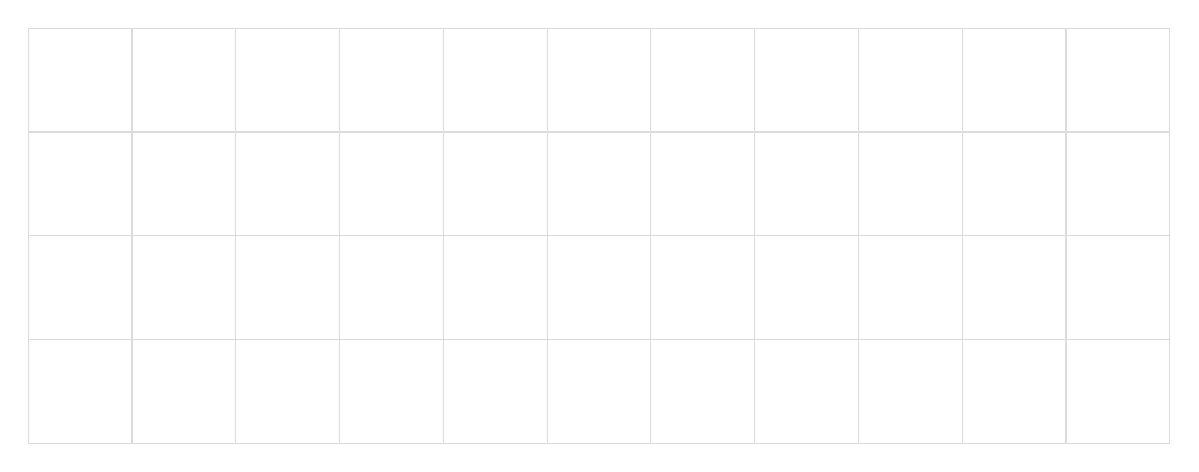
\begin{tikzpicture}[x=0.75pt,y=0.75pt,yscale=-1,xscale=1]
%uncomment if require: \path (0,208); %set diagram left start at 0, and has height of 208

%Shape: Grid [id:dp33505564538856114] 
\draw  [draw opacity=0] (2,2) -- (552,2) -- (552,202) -- (2,202) -- cycle ; \draw  [color={rgb, 255:red, 220; green, 220; blue, 220 }  ,draw opacity=1 ] (52,2) -- (52,202)(102,2) -- (102,202)(152,2) -- (152,202)(202,2) -- (202,202)(252,2) -- (252,202)(302,2) -- (302,202)(352,2) -- (352,202)(402,2) -- (402,202)(452,2) -- (452,202)(502,2) -- (502,202) ; \draw  [color={rgb, 255:red, 220; green, 220; blue, 220 }  ,draw opacity=1 ] (2,52) -- (552,52)(2,102) -- (552,102)(2,152) -- (552,152) ; \draw  [color={rgb, 255:red, 220; green, 220; blue, 220 }  ,draw opacity=1 ] (2,2) -- (552,2) -- (552,202) -- (2,202) -- cycle ;




\end{tikzpicture}

\fi

\begin{enumerate}

  \item[2.] Why does it not make sense to ask what the electric \emph{force} is at the origin?

            \ifsolutions
            Answer: There is no charge at the origin. (The electric field can be used to find the force on a charge \emph{if} it was placed at the origin.)
            \else

            \vskip 24pt
            \fi

\end{enumerate}

In the following, 

\begin{enumerate}

  \item[3.] Find the electric field at the origin due to $q_1$. Write your answer in the form $\bfvec{E}_1=E_{x1}\ihat + E_{y1}\jhat$.

            \ifsolutions
            {\bf Answer}: $\ds\bfvec{E}_1=-\frac{kq}{a^2}\ihat$
            \else

            \vskip 72pt
            \fi

  \item[4.] Find the electric field at the origin due to $q_2$. Write your answer in the form $\bfvec{E}_2=E_{x2}\ihat + E_{y2}\jhat$.

            \ifsolutions
            {\bf Answer}: $\ds\bfvec{E}_2=+\frac{kq}{a^2}\ihat$
            \else

            \vskip 72pt
            \fi

  \item[5.] Find the electric field at the origin due to $q_3$. Write your answer in the form $\bfvec{E}_3=E_{x3}\ihat + E_{y3}\jhat$.

            \ifsolutions
            {\bf Answer}: $\ds\bfvec{E}_3=+\frac{kq}{a^2}\jhat$
            \else

            \vskip 72pt
            \fi

  \item[6.] Find the total electric field at the origin by adding $\bfvec{E}_1$, $\bfvec{E}_2$, and $\bfvec{E}_3$. Write your answer in the form $\bfvec{E}=E_{x}\ihat + E_{y}\jhat$.

            \ifsolutions
            {\bf Answer}: $\ds\bfvec{E}=+\frac{kq}{a^2}\jhat$
            \else

            \vskip 72pt
            \fi

  \item[7.] Will your answers to 3.--6. change if the problem had asked for the electric field at a different position? If so, which answers?

            \ifsolutions
            Yes, all answers. The electric field at a given location due to each charge depends on the distance to the location. If the location changes, the distance changes.
            \else

            \vskip 72pt
            \fi

  \item[8.] Find the electric field at the origin if charge $q_1=2q$ (instead of $q$).

            \ifsolutions
            {\bf Answer}: $\ds\bfvec{E}=-\frac{kq}{a^2}\ihat+\frac{kq}{a^2}\jhat$
            \else

            \vskip 72pt
            \fi

  \item[9.] Find the electric field at the origin if charge $q_1=-2q$ (instead of $q$).

            \ifsolutions
            {\bf Answer}: $\ds\bfvec{E}=+\frac{3kq}{a^2}\ihat+\frac{kq}{a^2}\jhat$
            \else

            \vskip 72pt
            \fi

\end{enumerate}

\end{document}